\documentclass[a4paper, 12pt, oneside]{article}

%****************packages**************
\usepackage[french]{babel}
\usepackage[T1]{fontenc}
\usepackage{setspace}
\usepackage{hyperref}
\usepackage[top=2.5cm, bottom=2.5cm, left=2.5cm, right=2.5cm]{geometry}
\usepackage{graphicx}
\usepackage{amssymb}
\usepackage[squaren,Gray]{SIunits}
\usepackage{tabularx}
\usepackage{float}
\usepackage{comment}
\usepackage{layout}
\usepackage{pifont}
\usepackage{enumitem}
\usepackage{multicol}
\usepackage{wasysym}
\usepackage{amssymb}
\graphicspath{ {./images/} }
\frenchbsetup{StandardLists=true}
\usepackage{epstopdf}
\epstopdfsetup{outdir=images/converted_to_pdf} % Dossier de sortie des images converties
\usepackage{fancyhdr}
\usepackage{graphicx,lipsum,wrapfig}
\usepackage{csquotes}
\usepackage{biblatex}
\usepackage{marvosym}
\usepackage{booktabs}
\usepackage[table,xcdraw]{xcolor}
\addbibresource{sources.bib}


% fichier perso (à adapter suivant le rapport)
%%%%%%%  Constantes (à changer) %%%%%%%%


\newcommand{\nomAuteur}{Cardinale Adrien}

\newcommand{\titre}{Projet ProgConcur Phase 1}

\newcommand{\nbrprojet}{0} % numéro de laboratoire

\newcommand{\prof}{Zysman Eytan}

\newcommand{\assistant}{}

\newcommand{\classe}{classe}

\newcommand{\departement}{Département des Technologies industrielles (TIN)}

\newcommand{\cours}{ProgConcur}

\newcommand{\unitp}[1]{\ensuremath{\, \mathrm{#1}}}



%\setlength{\headheight}{27.06pt}
\pagestyle{fancy}

% Entête :
\fancyhead{} %remove header
\renewcommand{\headrulewidth}{0pt} % remove line

% Pied de page
\fancyfoot{} % clear all footer fields
\renewcommand{\footrulewidth}{0.5pt}
\fancyfoot[R]{Page \thepage}
\fancyfoot[L]{HEIG-VD | \nomAuteur }

%****************Document****************
\begin{document}
%\layout
    \begin{titlepage}
    \vfill
    
    \begin{center}
        
\includegraphics[height=2cm]{images/logo_heig.pdf}
        \hfill 
        
\includegraphics[height=2cm]{images/logo_hes-so.eps}
    \end{center}

    \vfill
    
    \begin{center}
        % \Large Laboratoire n°\nbrprojet:\\
        \huge  \textbf{\titre\\}
    \end{center}

    \begin{figure}[H]
        \centering
        
\includegraphics[scale=0.5]{images/un-bucheron-barbu-en-pin-up-pour-un-calendrier-1 (1).jpg}
    \end{figure}
    
    \begin{center}
        \begin{tabular}{l l}
             Département :         & \departement \\
             Unité d'enseignement : & \cours
        \end{tabular}
    \end{center}
    
    \vspace{1pt}
    
    % \vfill
    % \includegraphics[height = 8cm]{images/illustration.png}
    % \vfill
    
    \begin{center}
        \begin{tabular}{l l l l}
           Auteurs :    & \nomAuteur\\
           Professeur : & \prof\\
           %Assistant :  & \assistant\\
           %Classe :     & \classe\\
           Date :       & \today
        \end{tabular}
    \end{center}
    
    \vfill
    
\end{titlepage}
    \thispagestyle{empty}
    \tableofcontents
    \newpage
    \section{Cahier des charges}
    Le but de ce projet est de simuler le paysage d'une scierie composé d'une forêt ou un bucheron coupe du bois qu'il stocke dans des bennes, un transporteur qui
    transporte les bennes jusqu'à l'usine et d'un ouvrier qui vide les bennes, scie le bois et stocke les planches. Dans la phase 2, un carrefour est ajouté
    avec un flux de voiture qui le traverse et des clients peuvent aller acheter des planches au magasin de l'usine. Les principaux acteurs de cette simulation sont
    les suivants:
        \subsection{Benne}
            \begin{itemize}
                \item Transmission de la benne entre le bucheron et le transporteur.
                \item Transmission de la benne entre l'ouvrier et le transporteur.
                \item Il y a 3 bennes qui sont partagées entre le bucheron, le transporteur et l'ouvrier.
            \end{itemize} 
        \subsection{Ouvrier}
            L'ouvrier est composé des multiples threads qui symbolisent ses taches.
            \begin{itemize}
                \item Thread maître (gestion de tous les threads).
                \item Thread qui vide la benne (priorité 1).
                \item Thread qui scie les troncs (priorité 2).
                \item Thread qui stocke les planches (priorité 3). 
                \item Thread gestion des clients (phase 2).
            \end{itemize}
        \subsection{Bucheron}
            Le bucheron n'a qu'un seul thread qui lui permet de couper du bois.
            \begin{itemize}
                \item Coupe du bois.
                \item Transport du bois jusqu'à la benne.
                \item Dépose du bois dans la benne.
                \item Retourne en forêt.
            \end{itemize}
        \subsection{Transporteur}
            Le transporteur n'a qu'un seul thread qui définit son parcourt.
            \begin{itemize}
                \item Amarre une benne à l'usine.
                \item Roule vers la forêt.
                \item Désamarrer la benne dans la forêt.
                \item Amarre une benne en forêt.
                \item Rouler vers l'usine.
                \item Désamarrer la benne à l'usine.
            \end{itemize}
        \subsection{SuperTimer}
            Le supertimer est un thread qui s'occupe de la gestion du temps.
            \begin{itemize}
                \item Gestion de la densité de voiture dans le carrefour.
                \item Gestion de la période d'ouverture du service de vente.
                \item Gestion du temps de travail des threads. Un thread doit finir sa tâche avant de se terminer. 
            \end{itemize}
    \newpage
        \section{Architecture de l'application}
        \subsection{UML du programme}
        La structure générale du programme suit le diagramme de classes suivant. La classe racine est la simulation qui contient toutes les instances des différents acteurs.
        C'est dans la classe Simulation que sont crée les threads du bucheron, du transporteur et de l'ouvrier. Les classes forêt et usine sont uniquement des
        paysages elles n'ont aucune méthode et serve uniquement a stocker les bennes sur les parkings remplissage bennes et transport bennes pour la forêt, et 
        sur les parkings extraction bennes et transport bennes pour l'usine. L'usine contient aussi en plus 3 variables qui sont les bois à scier,
        les planches à stocker et le stock de planches. Le bucheron est associé à la forêt, car il peut remplir les bennes qui sont sur le parking remplissage
        et déplacer les bennes pleines sur le parking transport. L'ouvrier est associé à l'usine, car il peut remplir les bennes qui sont sur le parking extraction et
        il peut déplacer les bennes pleines sur le parking transport. Il a aussi accès aux différents stocks pour pouvoir scier le bois et stocker les planches. Le
        transporteur est associé à la forêt et à l'usine, car il peut amarrer une benne dans les parkings transport et il peut la désamarrer dans les parkings: 
        extraction et remplissage.
        Le thread du superTimer est instancié dans le main, il s'agit d'une classe singleton que tous les acteurs peuvent appeler pour connaitre l'heure actuelle.
        Le thread du superAffichage est aussi instancié dans le main et il s'agit d'une classe de singleton qui permet d'afficher les informations sur 
        l'interface graphique à l'aide de la bibliothèque SFML.
        \begin{figure}[H]
            \centering
            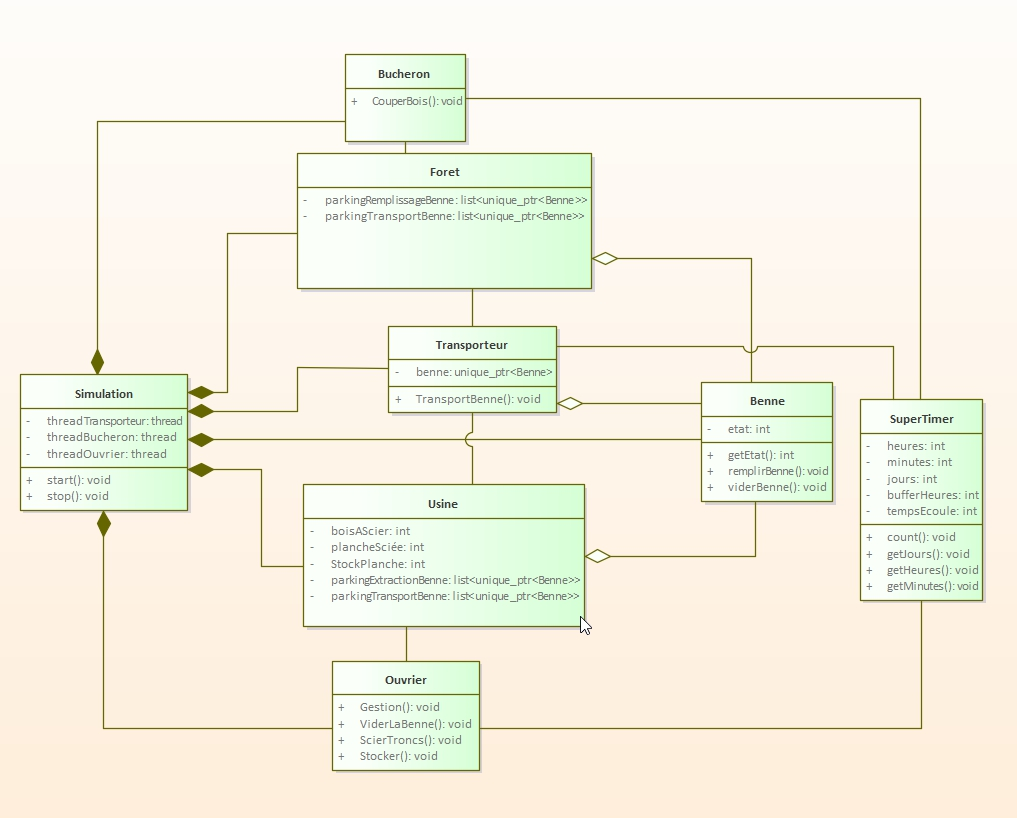
\includegraphics[scale=0.55]{images/uml phase 1.jpg}
            \caption{UML du programme}
        \end{figure}

        \subsection{Machine d'état du bucheron}
        Le bucheron est composé d'un seul thread qui a été programmé à partir de la machine d'état suivante:
        \begin{figure}[H]
            \centering
            \includegraphics[scale=0.7]{images/machine d'état bucheron.png}
            \caption{Machine d'état du bucheron}
        \end{figure}
         
        \newpage
        \subsection{Machines d'états ouvriers}
        L'ouvrier est composé d'un thread maître qui contrôle 3 threads qui sont les taches: vider la benne, scier du bois et stocker les planches. C'est
        le thread maître qui appelle les autres threads en fonction des taches à faire. Vider la benne est la tâche la plus prioritaire et stocker les planches 
        est la tâche la moins prioritaire. Ce choix est représenté par la machine d'état suivante:
        \begin{figure}[H]
            \centering
            \includegraphics[scale=0.7]{images/machine d'état gestion ouvrier.png}
            \caption{Machines d'état thread maître ouvrier}
        \end{figure}

        \newpage
        Les 3 taches de l'ouvrier (vider la benne, scier du bois et stocker les planches) sont programmées à partir de 3 machines d'état distinct, représenté à la 
        figure suivante, qui sont instanciées dans 3 threads séparés et qui sont appelées par le thread maître en fonction des tâches que l'ouvrier doit effectuer.
        \begin{figure}[H]
            \centering
            \includegraphics[scale=0.5]{images/machines d'état ouvrier.jpg}
            \caption{Machines d'états des threads ouvriers}
       \end{figure}

        \newpage
        \subsection{Machine d'état transporteur}
        Le transporteur est composé d'un thread programmé avec la machine d'état suivante:
        \begin{figure}[H]
            \centering
            \includegraphics[scale=0.7]{images/machine d'état transporteur.jpg}
            \caption{Machines d'état scieur}
        \end{figure}

        

    \newpage    
    \section{Mécanisme mis en jeu pour tous les aspects concurrents}
    Les bennes sont la seule ressource critique dont plusieurs threads peuvent avoir besoin. Les bennes sont stockées dans 4 vecteurs différents, ce qui limite le nombre
    d'interactions possible par les acteurs. Par exemple si la benne est sur le parking extraction, seul l'ouvrier y a accès pour la vider. Le transporteur peut
    uniquement en rajouter une dans la deque mais il ne peut pas retirer celle que l'ouvrier vider, car il ne peut retirer une benne que sur le parking de transport.
    Par contre, ce système peut bloquer un thread s’il n'y a pas de benne dans la deque où il doit accéder. Pour éviter qu'un thread ce bloque quand il n'a plus
    de benne, j'ai utilisé des variables de condition pour qu'un thread qui a besoin d'une benne non disponible puisse se mettre en wait. Quand un thread déplacer
    une benne dans une zone qui débloque l'autre thread, il le notifie pour qu'il puisse reprendre sa tache.
    \newpage
    \section{Réalisation}
    \subsection{Interface graphique}
    Pour ce projet, un de mes objectifs supplémentaires était d'avoir un retour visuel plus parlant que du texte dans un terminal. J'ai donc utilisé la bibliothèque 
    SFML pour créer une interface graphique.
    \begin{figure}[H]
        \centering
        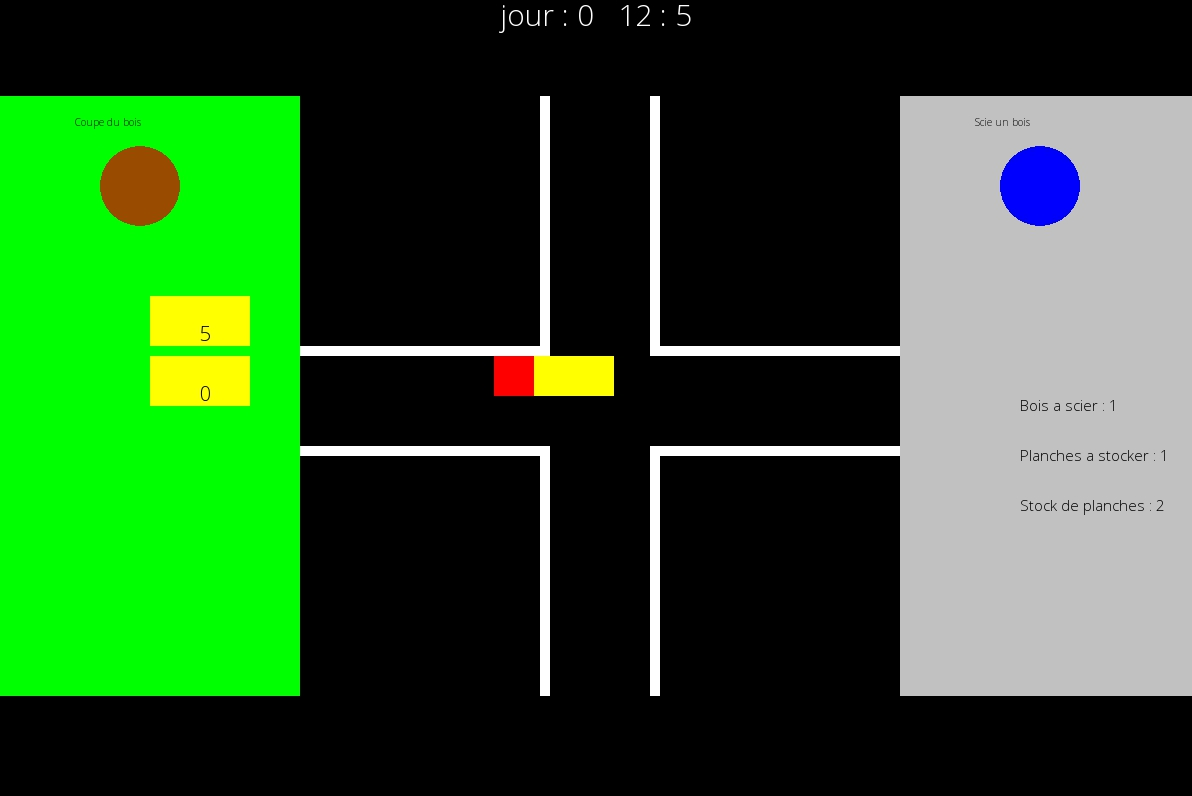
\includegraphics[scale=0.5]{images/interface graphique.jpg}
        \caption{Interface graphique}
    \end{figure}
    Cette interface me permet d'afficher le travail des différents acteurs et la position des bennes dans la simulation.

    \subsection{Choix du container}
    Pour ce projet, j'ai beaucoup hésité sur le choix des containers à utiliser pour stocker les bennes. Je suis en premier lieu parti sur des vecteurs, car il 
    permet d'ajouter des éléments dynamiquement dans un tableau. Mais il  permet d'ajouter et enlever des éléments qu’a la fin du tableau. Ce qui posait problème,
    car un thread pouvait travailler sur une benne et un autre pouvait lui en mettre une autre à la place. Il faut donc un container où un thread travaille sur le
    début de la file et dont l'autre ajoute des éléments à la fin de la file. Alors j'ai choisi d'utiliser des deques (file d'attente à double extrémité) qui 
    permettent un accès des 2 côtés de la file. Il existe aussi les queues qui auraient pu permettre un accès des 2 côtés de la file mais elles ne permettent pas l'accès
    au milieu de la file. Ce qui est nécessaire pour mon système d’affichage.
    
    \newpage
    \section{Conclusion}
    Cette première phase a demandé pas de mal de réflexion afin d'avoir tous les acteurs qui fonctionne en harmonie ensemble et permettre d'intégrer l'interface 
    graphique SFML. Je pense qu'il a fallu une bonne quinzaine d'heures pour arriver à la première phase de ce projet. 
    
    Pour la prochaine phase, j'aimerais améliorer les interactions entre les threads et le superTimer. Pour le moment, les threads font en permanence des requêtes au superTimer 
    pour connaitre l'heure actuelle. Pour la  prochaine phase, j'aimerais utiliser des variables de condition pour que les threads puissent se mettre en attente quand il n'est pas 
    l'heure de travailler.


\end{document}
